\documentclass{beamer}

\mode<presentation>
{
  \usetheme{Warsaw}
  \useoutertheme{infolines}
  \usecolortheme{spruce}
  % or ...

  \definecolor{beamer@verdeSoft}{rgb}{0.337,0.866,0.341}
  \definecolor{beamer@verdeDark}{rgb}{0.01,0.326,0.01}
  \setbeamercolor{item projected}{bg=green}
  \setbeamercolor{section in toc}{fg = beamer@verdeDark}
  \setbeamercolor{block title}{fg=beamer@verdeDark, bg = beamer@verdeSoft}
  %\setbeamercolor{local structure}{fg=green}

  \setbeamercovered{transparent}
  % or whatever (possibly just delete it)
}

\usepackage{hyperref}
\usepackage{multicol}
\usepackage{graphicx}
\usepackage{verbatim}
\usepackage{amsmath}
\usepackage{listings}
\usepackage{siunitx}
\usepackage{colortbl}

\lstloadlanguages{C++}
\lstnewenvironment{code}
	{%\lstset{	numbers=none, frame=lines, basicstyle=\small\ttfamily, }%
	 \csname lst@SetFirstLabel\endcsname}
	{\csname lst@SaveFirstLabel\endcsname}
\lstset{% general command to set parameter(s)
	language=C++, basicstyle=\footnotesize\sffamily, keywordstyle=\slshape,
	emph=[1]{tipo,usa}, emphstyle={[1]\sffamily\bfseries},
	morekeywords={tint,forn,forsn},
	basewidth={0.47em,0.40em},
	columns=fixed, fontadjust, resetmargins, xrightmargin=5pt, xleftmargin=15pt,
	flexiblecolumns=false, tabsize=2, breaklines,	breakatwhitespace=false, extendedchars=true,
	numbers=left, numberstyle=\tiny, stepnumber=1, numbersep=9pt,
	frame=l, framesep=3pt,
}

% Para mechar color en el texto
\lstset{escapeinside={<<<@}{@>>>}}

\usepackage[spanish]{babel}
% or whatever

\usepackage[utf8]{inputenc}
% or whatever

\usepackage{times}
\usepackage[T1]{fontenc}
% Or whatever. Note that the encoding and the font should match. If T1
% does not look nice, try deleting the line with the fontenc.


\title[Primalidad y Factorización] % (optional, use only with long paper titles)
{Primalidad y Factorización}

\author[Agustín Gutiérrez] % (optional, use only with lots of authors)
{~Agustín Santiago Gutiérrez}
% - Give the names in the same order as the appear in the paper.
% - Use the \inst{?} command only if the authors have different
%   affiliation.
\institute[UBA] % (optional, but mostly needed)
{
  Facultad de Ciencias Exactas y Naturales\\
  Universidad de Buenos Aires
}
\date[Camp 2016] % (optional, should be abbreviation of conference name)
{Campamento Caribeño ACM-ICPC 2016}

% Acá se puede insertar el logo de la UBA
% \pgfdeclareimage[height=0.5cm]{university-logo}{university-logo-filename}
% \logo{\pgfuseimage{university-logo}}



% Delete this, if you do not want the table of contents to pop up at
% the beginning of each subsection:
\AtBeginSubsection[]
{
  \begin{frame}{Contenidos}
  \footnotesize
    \tableofcontents[currentsection, currentsubsection]
  \end{frame}
}

\AtBeginSubsubsection[]
{
  \begin{frame}{Contenidos}
  \footnotesize
    \tableofcontents[currentsection, currentsubsection]
  \end{frame}
}

% If you wish to uncover everything in a step-wise fashion, uncomment
% the following command: 

%\beamerdefaultoverlayspecification{<+->}


\begin{document}

\begin{frame}
  \titlepage
\end{frame}

\begin{frame}{Contenidos}
  \tableofcontents
  % You might wish to add the option [pausesections]
\end{frame}



\section{Aritmética modular}

\newcommand{\modulo}[1]{\unaccentedoperators \pmod{#1}}

\subsection{Operaciones, estructura}

\begin{frame}{Definición}
  \begin{block}{Aritmética módulo $M$ ($\mathbb{Z}_M$)}
  La aritmética módulo $M$ consiste en una modificación de la aritmética usual de números enteros, en la cual trabajamos únicamente con el \textit{resto} de los números al ser divididos por un cierto entero fijo $M>0$,
  ignorando ``todo lo demás'' de los números involucrados.
  \end{block}
  \begin{itemize}
      \pause
      \invisible<1>{\item Así, $11 = 18$ si estamos trabajando módulo $7$, pues ambos dejan un resto de $4$ en la división por $7$. Esto se suele notar $11 \equiv 18 \modulo{7}$}
      \pause
      \invisible<1-2>{\item Una forma operacional de ver esta aritmética es suponer que todo el tiempo tenemos los números reducidos al rango de enteros en $[0,M)$, y tomamos el resto de la división por $M$ para devolverlos a ese rango luego de cada operación.}
  \end{itemize}
\end{frame}

\begin{frame}{Propiedades}
    A los efectos de realizar sumas, restas y productos, la aritmética módular es análoga a la aritmética usual, manteniendo sus propiedades importantes.
  \begin{itemize}
       \item $a+b \equiv b+a \modulo{M}$
       \item $(a+b)+c \equiv a+(b+c) \modulo{M}$
       \item $0$ es el neutro de la suma.
       \item Para todo $a$ existe un único inverso aditivo modular $-a$, $a + (-a) \equiv  0 \modulo{M}$. $a-b  \equiv  a + (-b) \modulo{M}$
       \item $a \cdot b \equiv b \cdot a \modulo{M}$
       \item $(a \cdot b) \cdot c \equiv a \cdot (b \cdot c) \modulo{M}$
       \item $1$ es el neutro del producto.
       \item $(a+b) \cdot c \equiv a \cdot c + b \cdot c \modulo{M}$
  \end{itemize}
\end{frame}


\begin{frame}[fragile]{Forma operacional en el código}
Supongamos que se tiene que computar una suma de los números enteros \texttt{a[0]} hasta \texttt{a[N-1]}, pero solamente nos importan los últimos 4 dígitos (equivale a trabajar módulo 10000).

\begin{columns}
\begin{column}{0.65\textwidth}
\begin{lstlisting}
int result = 0;
for (int i = 0; i < N; i++)
    result = (result + a[i]) % 10000;
\end{lstlisting}
\end{column}
\end{columns}

Como decíamos antes, a nivel de operaciones trabajar con aritmética modular equivale a simplemente tomar módulo luego de cada operación aritmética básica.

\end{frame}

\begin{frame}{Problema ante números negativos}
Sin embargo, la implementación anterior puede resultar problemática al trabajar con números \textbf{negativos}.

\begin{itemize}
    \item Si por ejemplo fuera $N=2$, \texttt{a[0]=123} y \texttt{a[1]=-200}, el código anterior produce -77, que puede no ser lo deseado.
    \item Incluso si no hay números negativos en el problema, es muy común que \textbf{restemos} números en nuestra solución.
    \item Estos resultados con valores negativos ocurren porque el resultado de la división entera se redondea hacia cero en los lenguajes y plataformas más populares.
    \pause
    \invisible<1-1>{\item Solución: \\ \texttt{int MOD(int x, int M)\{return ((x\%M)+M)\%M;\}} }
\end{itemize}

\end{frame}

\begin{frame}{Cuidado con el overflow}
\begin{itemize}
    \item Otro problema al que es especialmente común enfrentarse al trabajar con aritmética modular es el peligro de tener overflow en las operaciones.

    \item Por esto es que tomamos módulo luego de cada operación, y no solamente al final de todo el programa.
    
    \item Truquito en C++: Tener en cuenta el tipo \texttt{\_\_int128}, entero de 128 bits. No está presente en todo judge, pero puede ser muy útil cuando está disponible.

\end{itemize}
\end{frame}

\begin{frame}{¿Qué pasa con la división?}
\begin{itemize}
    \item ¿Podemos operar modularmente con la división tal cual lo hacemos con sumas, restas y productos?

    \pause
    \invisible<1-1>{
        \item \textbf{NO}. Por ejemplo: \\
             $\frac{10}{2}\equiv 5 \modulo{8}$, pero $10 \equiv 2 \modulo{8}$ y $\frac{2}{2} \equiv 1 \not\equiv 5 \modulo{8}$
        \item Podemos garantizar que este ``truco'' funciona cuando el módulo es un número \textbf{primo}. \\
             $\frac{27}{3}\equiv 2 \modulo{7}$, $27 \equiv 6 \modulo{7}$ y $\frac{6}{3} \equiv 2 \modulo{7}$ \\
             Pero solo si el divisor \textbf{no es cero} (módulo $p$) \\
             $\frac{140}{14}\equiv 3 \modulo{7}$, pero $140 \equiv 14 \equiv 0 \modulo{7}$ y $\frac{0}{0} \equiv ? \modulo{7}$ \\
        \pause
        \invisible<1-2>{
            \item ¿Pero y si aún con un módulo primo, la división modular no resulta una división entera? \\
                 $\frac{12}{3}\equiv 4 \modulo{7}$, pero $12 \equiv 5 \modulo{7}$ y $\frac{5}{3} \equiv ? \modulo{7}$ \\
        }
    }

\end{itemize}
\end{frame}

\begin{frame}{Inversos modulares}
    \begin{block}{Definición}
       Decimos que $b$ es inverso de $a$ módulo $M$ si $a \cdot b \equiv 1 \modulo{M}$.
    \end{block}
    Notar que solo un $a \not \equiv 0 \modulo{M}$ podría tener un inverso, y de existir el inverso es único, y a su vez $a$ resulta ser el inverso de $b$.
\pause
      \invisible<1>{
        \begin{block}{Teorema}
           Si $p$ es un número primo, entonces todo número $a \not \equiv 0 \modulo{p}$ tiene un inverso módulo $p$.
        \end{block}
        }

\end{frame}

\begin{frame}{Inversos modulares: utilidad}
    \begin{itemize}
        \item Recordemos que para realizar $3 / 2 = 1.5$, en realidad podríamos multiplicar directamente por el inverso de $2$, es decir $3 \cdot 0.5 = 1.5$
        \item Lo mismo podemos hacer modularmente. Por ejemplo, $5 \cdot 3 \equiv 1 \modulo{7}$, así que $inv(3)=5$. Y entonces recordando el ejemplo anterior:\\
               $\frac{12}{3}\equiv 4 \modulo{7}$, \\ $12 \equiv 5 \modulo{7}$ y \\$\mbox{``}\frac{5}{3}\mbox{''} \equiv 5 \cdot inv(3) \equiv 5 \cdot 5 \equiv 4 \modulo{7}$ 
        \item De esta forma, ya podemos dividir modularmente al trabajar con un número primo (excepto cuando el divisor se hace $0$ módulo $p$).
        \item ¿Pero cómo calculamos los inversos?
    \end{itemize}

\end{frame}

\subsection{Fermat e inversos modulares}

\begin{frame}{Pequeño teorema de Fermat}
  \begin{block}{Teorema}
  Si $p$ es primo y $a \not \equiv 0 \modulo{p}$, entonces $a^{p-1} \equiv 1 \modulo{p}$
  \end{block}
  \begin{itemize}
      \item Por ejemplo $6^{30} = 7131416765184947029025 \cdot 31 + 1$
      \item ¿Para qué puede servir este teorema?
  \end{itemize}
\end{frame}

\begin{frame}{Aplicación 1: Cálculo de inversos}
  \begin{itemize}
      \item Recordemos que dado $a \not \equiv 0$, si encontramos algún número $x$ tal que $a \cdot x \equiv 1 \modulo{p}$, $x$ será automáticamente el inverso de $a$.
      \item Si tomamos $x = a^{p-2}$, ¿Cuánto vale $a \cdot x$?
      \pause
      \invisible<1-1>{
        \item Tenemos $a \cdot x = a^{p-1} \equiv 1 \modulo{p}$ por el Pequeño Teorema de Fermat.
        \item Luego para cada $a$ su inverso será simplemente $a^{p-2}$.
      }
  \end{itemize}
\end{frame}

\begin{frame}{Aplicación 2: Testeo de residuo cuadrático}
  \begin{block}{Definición}
  Un resto $r$ se dice un \textit{residuo cuadrático} módulo $p$ si existe $x$ tal que $x^2 \equiv r \modulo{p}$
  \end{block}
  Por ejemplo los residuos cuadráticos módulo $5$ son $0,1,4$. Notar que $0$ siempre es residuo cuadrático módulo $p$.
  \begin{itemize}
          \item Si $r \not \equiv 0$ es residuo cuadrático, ¿Cuánto vale $r^{\frac{p-1}{2}}$?
          \pause
      \invisible<1-1>{
          \item $r \equiv x^2$ para algún $x \not \equiv 0$, y entonces $r^{\frac{p-1}{2}} \equiv (x^2)^{\frac{p-1}{2}} \equiv 1 \modulo{p}$
          \item Se puede verificar que además si para algún $r$ vale $r^{\frac{p-1}{2}} \equiv 1 \modulo{p}$, $r$ es residuo cuadrático módulo $p$.
      }
  \end{itemize}
\end{frame}

\subsection{Potenciación logarítmica}

\begin{frame}{Potenciación logarítmica}
  \begin{itemize}
      \item En los ejemplos anteriores hemos reducido algunos problemas a calcular $a^b$ módulo $M$, para enteros no negativos $a,b,M$.
      \item ¿Cómo hacemos esto más eficientemente que realizando $b-1$ multiplicaciones?
  \end{itemize}
\end{frame}

\begin{frame}{Potenciación logarítmica (idea)}
  \begin{itemize}
      \item Una buena idea es pensar en ir elevando al cuadrado sucesivamente, lo cual permite que el exponente crezca rápidamente.
      \item Pensado de manera recursiva, si llamamos $f(a,n) = a^n$: \\
              $\begin{array}{rcl}
                     f(a,n) & = & \left \{ \begin{array}{cl}
                                              1  & \mbox{si }n=0 \\
                                              f \left (a^2, \frac{n}{2} \right ) & \mbox{si } n \mbox{ es par} \\
                                              a \cdot f \left (a^2, \left \lfloor \frac{n}{2} \right \rfloor \right ) & \mbox{si } n \mbox{ es impar} \\
                                           \end{array} \right . \\
               \end{array}$
  \end{itemize}
\end{frame}


\begin{frame}[fragile]{Potenciación logarítmica (código)}
\begin{columns}
\begin{column}{0.60\textwidth}
\begin{lstlisting}
typedef long long tint;
tint potlog(tint a,tint b, const tint M)
{
    tint res = 1;
    while (b > 0)
    {
        if (b%  2 != 0)
            res = MOD(res*a, M);
        a = MOD(a*a, M);
        b /= 2;
    }
    return res;
}\end{lstlisting}
\end{column}
\begin{column}{0.45\textwidth}
Invariante de ciclo:

La respuesta que deseamos es $res \cdot (a^b \mbox{ módulo } M)$

Este método realiza solamente $O(\lg b)$ multiplicaciones.
\end{column}
\end{columns}
\end{frame}

\section{Primalidad}

\subsection{Criba}

\begin{frame}{Problema}
  \begin{itemize}
      \item Una necesidad muy usual al trabajar con números primos es la de calcular \textit{todos} los primos desde $1$ hasta $N$ para un cierto $N$.
      \item La idea es realizarlo de manera más eficiente que verificando la primalidad de cada número por separado.
  \end{itemize}
\end{frame}

\begin{frame}{Idea 1}
  \begin{itemize}
      \item Si verificásemos cada número por separado, lo que haríamos sería recorrer sus posibles \textbf{divisores} para ver si es primo.
      \item ¿Que pasaría si en lugar de probar los divisores de cada número, descartásemos sus \textbf{múltiplos}?
      \pause
      \invisible<1-1>{
           \item Hay $\frac{N}{1}$ múltiplos de $1$, $\frac{N}{2}$ múltiplos de $2$, $\cdots \frac{N}{N}$ múltiplos de $N$. Luego si recorremos todo
            el costo total es
            
            $$\sum_{i=1}^N{\frac{N}{i}} = N \sum_{i=1}^N{\frac{1}{i}} = \Theta(N \lg N)$$
      }
  \end{itemize}
\end{frame}

\begin{frame}[fragile]{Idea 1 (cont.)}
  \begin{itemize}
      \item Esta idea es verdaderamente muy sencilla, y como vimos ya alcanza una eficiencia aceptable.
      \item Además, al recorrer los múltiplos de todos los números, se encuentran todos los divisores propios de todos los números.
      \item De esta forma es extremadamente fácil modificar esta versión para computar fácilmente sumas de divisores, cantidades, y otras funciones similares.
  \end{itemize}

\begin{lstlisting}
    for(int i = 0; i < MAX; i++) p[i] = true;
    p[0] = p[1] = false;
    for (int i = 2; i < MAX; i++)
        for (int j = 2*i; j < MAX; j += i) p[j] = false;
\end{lstlisting}
\end{frame}

\begin{frame}[fragile]{Idea 2}
  \begin{itemize}
      \item Todo número compuesto tiene un divisor \textbf{primo}.
      \item Por lo tanto, alcanza con descartar los múltiplos de los números primos que vamos encontrando.
      \item La cantidad de operaciones a realizar en este caso se reduce a $\Theta(N \lg \lg N)$, que es ``casi lineal''.
  \end{itemize}

\begin{lstlisting}
    for(int i = 0; i < MAX; i++) p[i] = true;
    p[0] = p[1] = false;
    for (int i = 2; i < MAX; i++)
    <<<@\textcolor{red}{if (p[i])}@>>>
        for (int j = 2*i; j < MAX; j += i) p[j] = false;
\end{lstlisting}
\end{frame}

\begin{frame}[fragile]{Idea 3}
  \begin{itemize}
      \item Todo número compuesto tiene un divisor primo $p$, con $p \leq \sqrt{N}$ .
      \item Podemos parar el proceso de descarte de múltiplos en $\sqrt{N}$.
      \item La cantidad de operaciones sigue siendo $\Theta(N \lg \lg N)$.
  \end{itemize}

\begin{lstlisting}
    for(int i = 0; i < MAX; i++) p[i] = true;
    p[0] = p[1] = false;
    for (int i = 2; <<<@\textcolor{red}{i*i}@>>> < MAX; i++)
    if (p[i])
        for (int j = 2*i; j < MAX; j += i) p[j] = false;
\end{lstlisting}
\end{frame}

\begin{frame}[fragile]{Idea 4}
  \begin{itemize}
      \item De manera similar al caso anterior, si $N < p^2$ es compuesto, tiene un divisor primo menor que $p$, y ya habrá sido descartado.
      \item Podemos comenzar el descarte de los múltiplos de $i$ por $i^2$.
      \item Aún con esta optimización, la cantidad de operaciones sigue siendo $\Theta(N \lg \lg N)$.
  \end{itemize}

\begin{lstlisting}
    for(int i = 0; i < MAX; i++) p[i] = true;
    p[0] = p[1] = false;
    for (int i = 2; i*i < MAX; i++)
    if (p[i])
        for (int j = <<<@\textcolor{red}{i*i}@>>>; j < MAX; j += i) p[j] = false;
\end{lstlisting}
\end{frame}


\begin{frame}{Tiempos}
     Para \texttt{MAX=300M}:
     
     $$\begin{array}{rl}
           \mbox{\texttt{RecorrerMultiplos}} & \SI{39.1}{\second} \\
           \mbox{\texttt{CribaBasica}} & \SI{5.6}{\second} \\
           \mbox{\texttt{CribaHastaRaiz}} & \SI{3.2}{\second} \\
           \mbox{\texttt{CribaHastaRaizDesdeICuadrado}} & \SI{3.0}{\second} \\
       \end{array}$$
\end{frame}


\subsection{Verificación directa}

\subsubsection{Algoritmo ingenuo}

\begin{frame}{Algoritmo ingenuo}
  \begin{itemize}
      \item Como ya hemos mencionado, un número compuesto $N$ tendrá un divisor primo menor o igual a $\sqrt{N}$
      \item Un algoritmo simple $O(\sqrt{N})$ consistirá entonces de un chequeo de todos los números enteros en el rango $[2, \sqrt{N}]$,
             en busca de divisores de $N$.
  \end{itemize}
\end{frame}


\subsubsection{Test de Rabin - Miller}

\begin{frame}{Test de Rabin - Miller (Introducción)}
  \begin{itemize}
      \item El test de Rabin-Miller es un algoritmo \textbf{probabilístico}, muy eficiente para verificar si un número es primo.
      \item Se basa en su antecesor, el \textit{test de Fermat}.
      \item Recordemos: $a \not\equiv 0 \modulo{p} \Rightarrow a^{p-1} \equiv 1 \modulo{p}$
  \end{itemize}
\end{frame}

\begin{frame}{Test de Fermat}
  \begin{itemize}
      \item El test de Fermat es un test probabilístico para verificar si un número candidato $N$ es primo.
      \item Se selecciona para ello un entero al azar $a \in [1, N)$.
      \item Si $N$ es primo necesariamente será $a^{N-1} \equiv 1 \modulo{N}$, así que si esto no ocurre descartamos al número como primo.
      \item Si esto ocurre, el número pasó el test de Fermat con $a$ como testigo. El test puede repetirse con varios valores de $a$ para aumentar la confianza.
  \end{itemize}
\end{frame}

\begin{frame}{Test de Fermat: problema}
  \begin{itemize}
      \item El test de Fermat es eficiente, pero tiene un problema: existen ejemplos de números que pasan el test de Fermat para todo valor de $a$ coprimo con $N$, pero que son compuestos.
      \item Estos números extremos son raros y se denominan de \textit{Carmichael}. Los primeros son 561, 1105, 1729, 2465, 2821, 6601, 8911.
      \item Con estos números, el test solamente los detecta como compuestos si $a$ es múltiplo de uno de los primos que dividen a $N$, y por lo tanto el test es prácticamente una búsqueda de divisores aleatoria.
  \end{itemize}
\end{frame}

\begin{frame}{Test de Rabin - Miller (idea)}
  \begin{itemize}
      \item El test de Rabin-Miller elimina este problema verificando una condición más fuerte.
      \item Observemos que si $p > 2$ es primo y $x^2 = 1 \modulo{p}$, $x$ solo puede ser $1$ o $-1$ módulo $p$.
      \item Luego si $p-1 = 2^\alpha k$, con $k$ impar y $\alpha \geq 1$, tenemos que para cualquier $a \not \equiv 0 \modulo{p}$ debe ser $a^{2^\alpha k} \equiv 1 \modulo{p}$.
      \item Pero entonces $a^{2^{\alpha-1} k} \equiv 1 \mbox{ o } -1 \modulo{p}$
      \item Y si fuera $1$, entonces nuevamente $a^{2^{\alpha-2} k} \equiv 1 \mbox{ o } -1 \modulo{p}$
      \item Y así podemos repetir el razonamiento hasta que $a^{k} \equiv 1$ o bien $a^{2^j k} \equiv -1$ para algún $0 \leq j < \alpha$
  \end{itemize}
\end{frame}

\begin{frame}{Test de Rabin - Miller (idea cont.)}
  Tenemos entonces las siguientes posibilidades para el valor de $a^{2^jk}$ (una por columna):
  $$\begin{array}{rccccccc}
      \mathbf{j} & \  & \ & \   & \ & \ & \  \\
      \alpha & 1 & 1 & \cdots & 1 & 1 & 1 & 1  \\
      \alpha-1 & -1 & 1 & \cdots & 1 & 1 & 1 & 1     \\
      \alpha-2 & ? & -1 & \cdots & 1 & 1 & 1 & 1    \\
      \cdots & \cdots & \cdots & \cdots & \cdots  & \cdots & \cdots &  \cdots    \\
      2 & ? & ? & \cdots & -1 &  1 & 1  & 1\\
      1 & ? & ? & \cdots &  ? & -1 & 1  & 1 \\
      0 & ? & ? & \cdots &  ? &  ? & -1 & 1 \\
    \end{array}
  $$
\end{frame}

\begin{frame}{Test de Rabin - Miller (implementación)}
  En general estas son chequeadas desde abajo hacia arriba, de forma que cada valor necesario es el cuadrado del que se necesitó en el paso anterior:
  $$\begin{array}{rccccc>{\columncolor{blue!30}}c>{\columncolor{blue!30}}cl}
      \mathbf{j} & \  & \ & \   & \ & \ & \ & \\
      \alpha & 1 & 1 & \cdots & 1 & 1 & 1 & 1 & \\
      \alpha-1 & -1 & 1 & \cdots & 1 & 1 & 1 & 1 &    \\
      \alpha-2 & ? & -1 & \cdots & 1 & 1 & 1 & 1 &   \\
      \cdots & \cdots & \cdots & \cdots & \cdots  & \cdots & \cdots &  \cdots &   \\
      2 & ? & ? & \cdots & -1 &  1 & 1  & 1 &\\
      1 & ? & ? & \cdots &  ? & -1 & 1  & 1 & \\
      0 & ? & ? & \cdots &  ? &  ? & -1 & 1 & \cellcolor{blue!30} a^k \equiv 1 \mbox{ o } -1 \\
    \end{array}
  $$
\end{frame}

\begin{frame}{Test de Rabin - Miller (implementación)}
  En general estas son chequeadas desde abajo hacia arriba, de forma que cada valor necesario es el cuadrado del que se necesitó en el paso anterior:
  $$\begin{array}{rcccc>{\columncolor{blue!30}}cccl}
      \mathbf{j} & \  & \ & \   & \ & \ & \ & \\
      \alpha & 1 & 1 & \cdots & 1 & 1 & 1 & 1 & \\
      \alpha-1 & -1 & 1 & \cdots & 1 & 1 & 1 & 1 &    \\
      \alpha-2 & ? & -1 & \cdots & 1 & 1 & 1 & 1 &   \\
      \cdots & \cdots & \cdots & \cdots & \cdots  & \cdots & \cdots &  \cdots &   \\
      2 & ? & ? & \cdots & -1 &  1 & 1  & 1 &\\
      1 & ? & ? & \cdots &  ? & -1 & 1  & 1 & \cellcolor{blue!30} a^{2k} = (a^{k})^2 \equiv -1\\
      0 & ? & ? & \cdots &  ? &  ? & -1 & 1 & \\
    \end{array}
  $$
\end{frame}

\begin{frame}{Test de Rabin - Miller (implementación)}
  En general estas son chequeadas desde abajo hacia arriba, de forma que cada valor necesario es el cuadrado del que se necesitó en el paso anterior:
  $$\begin{array}{rccc>{\columncolor{blue!30}}ccccl}
      \mathbf{j} & \  & \ & \   & \ & \ & \ & \\
      \alpha & 1 & 1 & \cdots & 1 & 1 & 1 & 1 & \\
      \alpha-1 & -1 & 1 & \cdots & 1 & 1 & 1 & 1 &    \\
      \alpha-2 & ? & -1 & \cdots & 1 & 1 & 1 & 1 &   \\
      \cdots & \cdots & \cdots & \cdots & \cdots  & \cdots & \cdots &  \cdots &   \\
      2 & ? & ? & \cdots & -1 &  1 & 1  & 1 & \cellcolor{blue!30} a^{2^2k} = (a^{2k})^2 \equiv -1\\
      1 & ? & ? & \cdots &  ? & -1 & 1  & 1 & \\
      0 & ? & ? & \cdots &  ? &  ? & -1 & 1 & \\
    \end{array}
  $$
\end{frame}

\begin{frame}{Test de Rabin - Miller (implementación)}
  En general estas son chequeadas desde abajo hacia arriba, de forma que cada valor necesario es el cuadrado del que se necesitó en el paso anterior:
  $$\begin{array}{rc>{\columncolor{blue!30}}ccccccl}
      \mathbf{j} & \  & \ & \   & \ & \ & \ & \\
      \alpha & 1 & 1 & \cdots & 1 & 1 & 1 & 1 & \\
      \alpha-1 & -1 & 1 & \cdots & 1 & 1 & 1 & 1 &    \\
      \alpha-2 & ? & -1 & \cdots & 1 & 1 & 1 & 1 & \cellcolor{blue!30} a^{2^{\alpha-2}k} \equiv -1   \\
      \cdots & \cdots & \cdots & \cdots & \cdots  & \cdots & \cdots &  \cdots &   \\
      2 & ? & ? & \cdots & -1 &  1 & 1  & 1 & \\
      1 & ? & ? & \cdots &  ? & -1 & 1  & 1 & \\
      0 & ? & ? & \cdots &  ? &  ? & -1 & 1 & \\
    \end{array}
  $$
\end{frame}

\begin{frame}{Test de Rabin - Miller (implementación)}
  En general estas son chequeadas desde abajo hacia arriba, de forma que cada valor necesario es el cuadrado del que se necesitó en el paso anterior:
  $$\begin{array}{r>{\columncolor{blue!30}}cccccccl}
      \mathbf{j} & \  & \ & \   & \ & \ & \ & \\
      \alpha & 1 & 1 & \cdots & 1 & 1 & 1 & 1 & \\
      \alpha-1 & -1 & 1 & \cdots & 1 & 1 & 1 & 1 & \cellcolor{blue!30} a^{2^{\alpha-1}k} \equiv -1   \\
      \alpha-2 & ? & -1 & \cdots & 1 & 1 & 1 & 1 &   \\
      \cdots & \cdots & \cdots & \cdots & \cdots  & \cdots & \cdots &  \cdots &   \\
      2 & ? & ? & \cdots & -1 &  1 & 1  & 1 & \\
      1 & ? & ? & \cdots &  ? & -1 & 1  & 1 & \\
      0 & ? & ? & \cdots &  ? &  ? & -1 & 1 & \\
    \end{array}
  $$
\end{frame}

\begin{frame}{Test de Rabin - Miller (conclusión)}
    \begin{itemize}
      \item Si ninguno de los casos anteriores se da, concluímos que definitivamente el número no es primo.
      \item Si alguno funciona, ese valor de $a$ funciona y el número parece ser primo.
      \item Al igual que en el test de Fermat, conviene utilizar varios valores de $a$ para aumentar la confianza.
      \item En el caso del test de Rabin-Miller, tenemos la garantía de que si $N$ es compuesto, al menos el 75\% de los posibles restos $a$ no nulos módulo $N$ lo demostrarán usando el test.
      \item Por lo tanto si repetimos el test $k$ veces sobre un número compuesto, eligiendo números de manera aleatoria, uniforme e independiente, la probabilidad de error es como máximo $\frac{1}{4^k}$.
      \item Los números primos siempre pasan el test, y son reportados como tales.
  \end{itemize}
\end{frame}

\begin{frame}{Test de Rabin - Miller (bonus)}
    \begin{itemize}
      \item Si los números a verificar no son demasiado grandes, se conocen versiones deterministas del test probando con un conjunto específico de valores de $a$.
      \item Por ejemplo wikipedia menciona:
        \begin{itemize}
          \item if n < 4,759,123,141 $>2^{32}$, it is enough to test: \\ a = 2, 7, and 61;
          \item if n < 18,446,744,073,709,551,616 = $2^{64}$, it is enough to test: \\a = 2, 3, 5, 7, 11, 13, 17, 19, 23, 29, 31, and 37.
        \end{itemize}
      \item Los artículos citados son:
        \begin{itemize}
          \item Jaeschke, Gerhard (1993), ``On strong pseudoprimes to several bases'', Mathematics of Computation 61 (204): 915-926
          \item Jiang, Yupeng; Deng, Yingpu (2014). ``Strong pseudoprimes to the first eight prime bases''. Mathematics of Computation 83 (290): 2915-2924. doi:10.1090/S0025-5718-2014-02830-5
        \end{itemize}
  \end{itemize}
\end{frame}





\section{Factorización}

\subsection{Criba}

\begin{frame}[fragile]{Factorización logarítmica}
  \begin{itemize}
      \item Buena alternativa si nos interesa poder factorizar rápidamente cualquier número hasta $N$, y aceptamos el costo de una criba hasta $N$.
      \item Si en lugar de solamente guardar si un número es primo o no, guardamos un primo que lo divida mientras hacemos la criba, luego podemos saber un divisor primo de cualquier número en $O(1)$. Esto permite factorizar cualquier número en $O(\lg N)$.
  \end{itemize}

\begin{lstlisting}
    for(int i = 0; i < MAX; i++) p[i] = i;
    p[0] = p[1] = 1;
    for (int i = 2; i*i < MAX; i++)
    if (p[i] == i)
        for (int j = i*i; j < MAX; j += i) p[j] = i;
\end{lstlisting}
\end{frame}

\subsection{Factorización directa}

\subsubsection{Algoritmo ingenuo}

\begin{frame}[fragile]{Algoritmo ingenuo}
  \begin{itemize}
      \item Sabemos que si no hay ningún factor primo hasta $\sqrt{N}$, $N$ debe ser primo.
      \item En virtud de esto, es natural dar un algoritmo de factorización que pruebe todos los posibles factores hasta ese valor.
      \item Notar que podemos cortar en la raíz de la parte de $N$ que falta factorizar, acelerando el proceso cuando hay bastantes factores chicos y uno grande.
      \item El peor caso sigue siendo $\Theta(\sqrt{N})$
  \end{itemize}

\begin{lstlisting}
    for(int i = 2; i*i <= N; i++)
    while (N % i == 0)
    {
        N /= i;
        reportarFactorPrimo(i);
    }
    if (N > 1)
        reportarFactorPrimo(N);
\end{lstlisting}
\end{frame}

\subsubsection{Algoritmo de la liebre y la tortuga de Floyd}

\begin{frame}{Introducción}
    \begin{block}{Problema}
        Supongamos que tenemos una sucesión $x_1, x_2, x_3, \cdots$ 
        
        Queremos ir leyéndola hasta encontrar la primera repetición (es decir, los menores $i,j$ tales que $x_i=x_j$ con $i < j$).
    \end{block}
    \begin{itemize}
      \item ¿Cómo podemos resolver esta tarea?
      \pause
      \invisible<1-1>{
         \item Árbol binario de búsqueda
         \item Tabla hash.
         \item Lista de valores
      }
    \end{itemize}
\end{frame}

\begin{frame}{Introducción (cont.)}
    \begin{itemize}
         \item Un árbol binario de búsqueda (\texttt{set} de C++, \texttt{TreeSet} de Java) es una estructura eficiente que lo resuelve en $O(j \lg j)$.
         \item Requiere $O(j)$ memoria.
         \item Requiere un operador $<$ para los valores.
    \end{itemize}
\end{frame}

\begin{frame}{Introducción (cont.)}
    \begin{itemize}
         \item Una tabla hash (\texttt{unordered\_set} de C++, \texttt{HashSet} de Java) es una estructura eficiente que lo resuelve en $O(j)$ (\textbf{asumiendo una buena función de Hash}).
         \item Requiere $O(j)$ memoria.
         \item Requiere que se pueda computar una función de hash sobre cada valor.
    \end{itemize}
\end{frame}

\begin{frame}{Introducción (cont.)}
    \begin{itemize}
         \item Una simple lista de valores (\texttt{vector} de C++, \texttt{ArrayList} de Java) es una estructura que lo resuelve en $O(j^2)$.
         \item Requiere $O(j)$ memoria.
         \item Únicamente requiere un operador de igualdad ($=$) sobre los elementos.
    \end{itemize}
\end{frame}

\begin{frame}{Introducción (cont.)}
    \begin{itemize}
    \item En el caso general (si leemos los $x_i$ de la entrada) es difícil mejorar estas estructuras. 
    \item Sin embargo, un caso muy común se da cuando la sucesión se obtiene por aplicación reiterada de alguna función $f$:\\
             $x_1$, $f(x_1)$, $f(f(x_1))$, $f(f(f(x_1)))$, $\cdots$
    \item Veremos un algoritmo para dicho caso particular, que logrará lo mejor entre todos ellos y más:
        \begin{itemize}
             \item O(1) memoria
             \item O(j) tiempo (u $O(j)$ aplicaciones de $f$ si el costo de $f$ no es $O(1)$)
             \item \textbf{Únicamente requiere un operador de igualdad ($=$) sobre los elementos}
        \end{itemize}
    \end{itemize}
\end{frame}

\begin{frame}{Estructura de $\rho$}
    \begin{itemize}
    \item En este caso, cuando aparezca la primera repetición $x_i = x_j$, necesariamente será $x_{i+1} = f(x_i) = f(x_j) = x_{j+1}$ y la secuencia entra en un ciclo
     de período $j-i$ que comienza en $i$.
     \item Gráficamente ($i=1785$, $j=3570$):
    \end{itemize}
    {\hfill 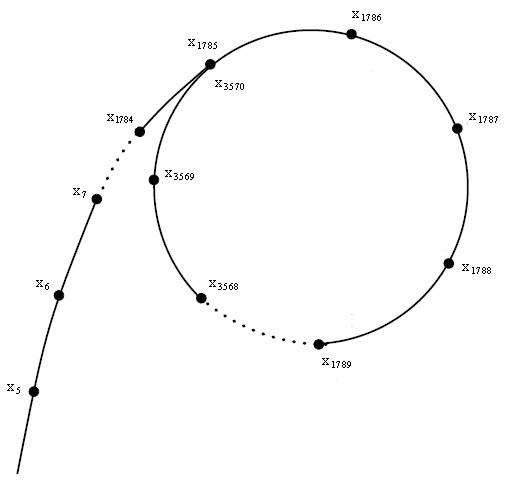
\includegraphics[scale=0.5]{rho_cycle.jpg} \hfill}
\end{frame}


\begin{frame}{Caso aún más particular}
    \begin{itemize}
    \item Cuando la $f$ es inversible, no es difícil ver que la primera repetición será de la forma $i=1$, $x_1 = x_j$.
    \item En efecto, si $f$ es inversible, la $\rho$ debe degenerar a un ciclo simple, pues de lo contrario $x_i$ tendría
           dos antecesores por $f$, y eso no puede ocurrir.
    \item El algoritmo para este caso sencillo es entonces aplicar $f$ sucesivas veces hasta encontrar un elemento tal que $x_j = x_1$.
    \end{itemize}
\end{frame}

\begin{frame}{Algoritmo de la liebre y la tortuga de Floyd}
    \begin{itemize}
    \item La idea en este caso es tener dos punteros, $a=x_2$ que será la tortuga y $b=x_3$ que será la liebre.
    \item $a$ avanzará de a un elemento, recorriendo toda la secuencia.
    \item $b$ en cambio avanzará de a \textbf{dos} elementos.
    \item En cada paso verificamos si $x_a = x_b$ y continuamos hasta que así sea.
    \item Notar que luego de $i$ pasos (no conocemos $i$), la tortuga y la liebre estarán ambos en el ciclo (digamos en $a_0=i$ y $b_0$).
    \item Luego de eso, en a lo más $j-i=T$ pasos más coincidirán (su diferencia se incrementa en 1 cada paso).
    \item Notar que si solamente nos interesa encontrar \textbf{alguna} coincidencia, podemos terminar aquí.
    \end{itemize}
\end{frame}

\begin{frame}{Algoritmo de la liebre y la tortuga de Floyd (cont)}
    \begin{itemize}
    \item Luego de $i=1784$ pasos. $a_0=1785$ y $b_0=1787$. Llamemos $d=b_0-a_0=2$.
    \end{itemize}
    {\hfill 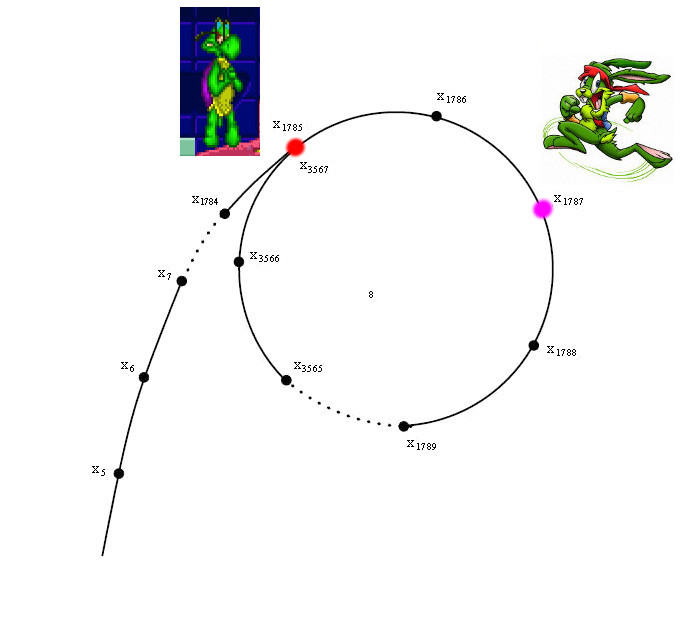
\includegraphics[scale=0.35]{hare_tortoise_rho_cycle1.jpg} \hfill}
\end{frame}

\begin{frame}{Algoritmo de la liebre y la tortuga de Floyd (cont)}
    \begin{itemize}
    \item Como en cada paso adicional la liebre se acerca en 1 a la tortuga, la alcanza luego de $T-d = 1780$ pasos más. Notar que se encuentran a $d$ del comienzo del ciclo.
    \end{itemize}
    {\hfill 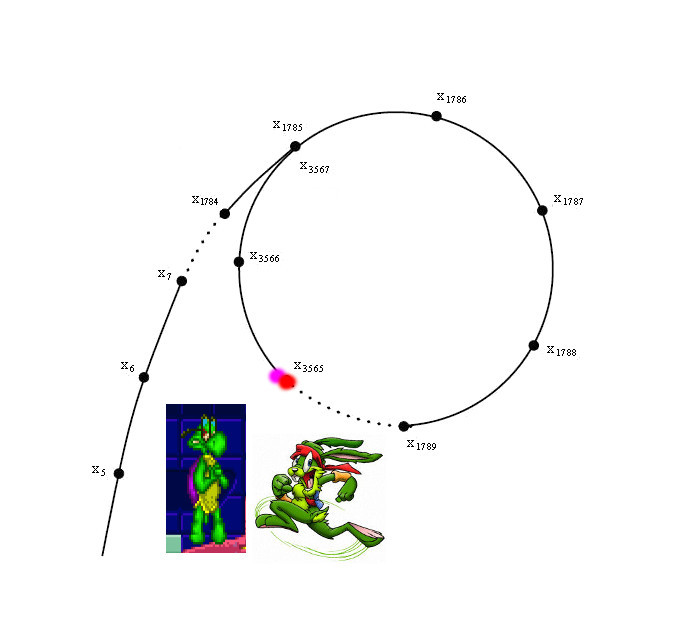
\includegraphics[scale=0.35]{hare_tortoise_rho_cycle2.jpg} \hfill}
\end{frame}

\begin{frame}{Algoritmo de la liebre y la tortuga de Floyd (cont)}
    \begin{itemize}
    \item Para completar el algoritmo, una vez que se encuentran ambos, reinicializamos la liebre (o la tortuga, da igual) al origen, y además, ahora hacemos moverse a la liebre de a un solo paso por vez, igual que la tortuga.
    \end{itemize}
    {\hfill 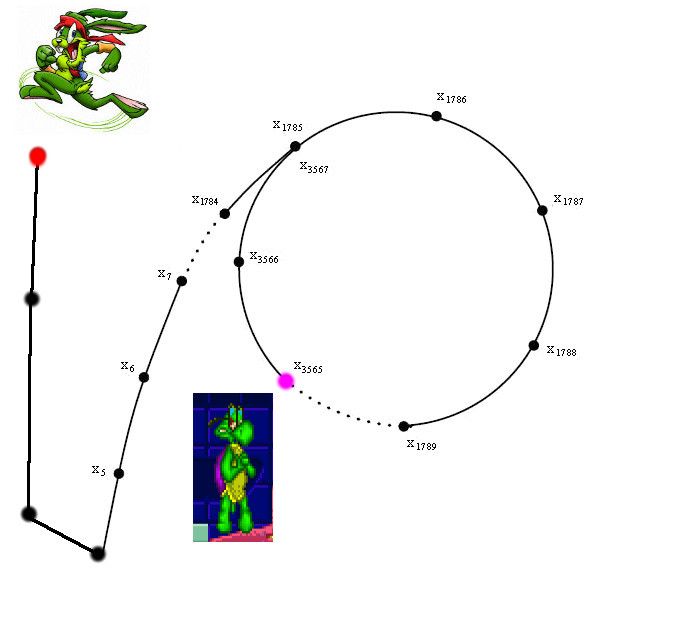
\includegraphics[scale=0.35]{hare_tortoise_rho_cycle3.jpg} \hfill}
\end{frame}

\begin{frame}{Algoritmo de la liebre y la tortuga de Floyd (cont)}
    \begin{itemize}
    \item $i$ pasos más tarde, ambos estarán en $x_i$, que será el nuevo punto de encuentro. Una vez allí, es fácil dejar uno fijo y dar una vuelta al ciclo con el otro para determinar su longitud. La cantidad total de pasos es como mucho $2j$.
    \end{itemize}
    {\hfill 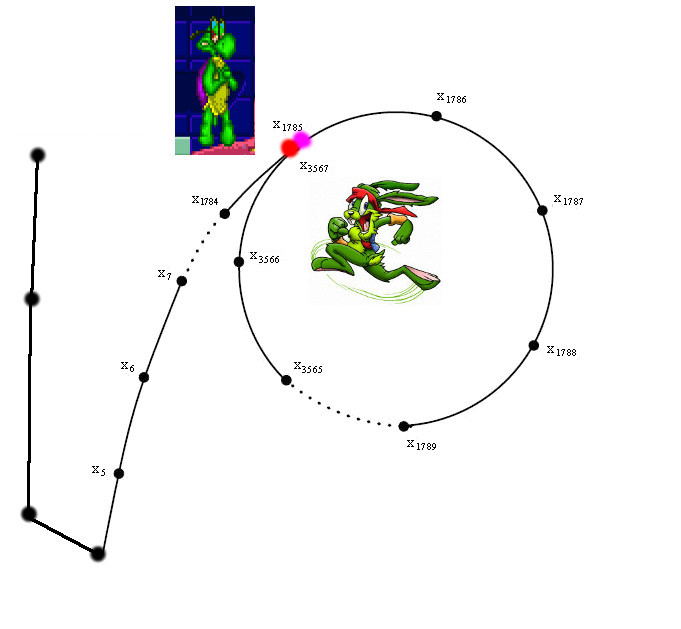
\includegraphics[scale=0.35]{hare_tortoise_rho_cycle4.jpg} \hfill}
\end{frame}

\begin{frame}{Alternativa}
    \begin{itemize}
    \item Una alternativa menos mencionada en la literatura, pero con mejores factores constantes (aunque idénticas complejidades asintóticas) es el algoritmo de Brent.
    \item Este se basa en ir duplicando la longitud de ciclo candidata en cada paso. Se puede leer sobre él en wikipedia (\textit{Brent's Cycle Detection}).
    \end{itemize}
\end{frame}

\subsubsection{Factorización rápida}

\begin{frame}{Paradoja de los cumpleaños}
    \begin{itemize}
      \item ¿Cuál es la probabilidad de que dos personas cumplan años el mismo día, en una sala con 23 personas?
      \pause
      \invisible<1-1>{
          \item 50.7\%
          \pause
          \invisible<1-2>{
              \item En general, dado un universo de $n$ objetos, la cantidad de elementos que hay que sacar al azar hasta que la probabilidad de que dos sean iguales
                 sea al menos 50\% es $\left \lceil \sqrt{2n \ln 2} \right \rceil + \epsilon$ , donde $\epsilon \in \{ 0, 1 \}$
              \item Similarmente, la cantidad esperada de elementos que hay que sacar al azar hasta que aparezca una primera repetición es
                    $\sqrt{\frac{\pi n}{2}} + \frac{2}{3} + \epsilon$ , donde $|\epsilon| \leq 1$  (Ramanujan, Watson y Knuth).
              \pause
              \invisible<1-3>{
                  \item \textbf{En resumen}, son $O(\sqrt{n})$ pasos hasta la primera repetición.
              }
          }
      }
    \end{itemize}
\end{frame}


\begin{frame}{Algoritmo de la $\rho$ de Pollard}
    \begin{itemize}
      \item Asumimos que $N$ es compuesto (podemos comenzar verificando su primalidad con algún test rápido como Rabin-Miller).
      \item La idea es aprovechar la paradoja de los cumpleaños para encontrar un factor propio de $N$ rápidamente.
      \item Una vez que encontramos un factor de $N$, basta repetir el procedimiento recursivamente hasta descomponer a $N$ en primos.
    \end{itemize}
\end{frame}

\begin{frame}{Algoritmo de la $\rho$ de Pollard (cont.)}
    \begin{itemize}
      \item Supongamos que $p \leq \sqrt{N}$ es un primo que divide a $N$.
      \item Si vamos generando números entre $1$ y $N-1$ al azar, sus restos módulo $p$ también serán aleatorios.
      \item La cantidad de pasos esperados hasta que se repita un valor módulo $N$ es $\Theta(\sqrt{N})$.
      \item Pero la cantidad de pasos esperados hasta que se repita un valor módulo $p$ es $\Theta(\sqrt{p}) = O(\sqrt[4]{N})$
      \item Luego esperamos que exista una repetición módulo $p$ rápidamente, antes de que haya una repetición módulo $N$.
      \pause
      \invisible<1-1>{
         \item ¿Pero cómo detectamos esta repetición, \textbf{si no conocemos $p$ a priori}?
      }
    \end{itemize}
\end{frame}

\begin{frame}[fragile]{Algoritmo de la $\rho$ de Pollard (cont.)}
    \begin{itemize}
      \item Si $x$ e $y$ son dos valores de nuestra secuencia que coinciden módulo $p$, $x-y \equiv 0 \modulo{p}$
      \item ¡ Entonces $p | MCD(|x-y|,N)$ !
      \item Este MCD puede calcularse con el algoritmo de Euclides sin conocer $p$.
      \begin{itemize}
           \item Si da $1 < MCD < N$, hemos encontrado un factor de $N$.
           \item Si da $MCD=N$, hemos tenido una repetición en la secuencia módulo $N$.
           \item Si da $MCD=1$, no hemos detectado ninguna repetición módulo $p$.
      \end{itemize}
      
           \texttt{int mcd(int a,int b) \\ \{return (a == 0) ? b : mcd(b\%a, a) ;\} }
           
    \end{itemize}
\end{frame}

\begin{frame}{Algoritmo de la $\rho$ de Pollard (cont.)}
    \begin{itemize}
      \item Notar que con este truco podemos verificar si $x$ e $y$ dados son coincidentes módulo algún $p$.
      \item Es decir, a la hora de buscar repeticiones en nuestra secuencia, \textbf{solamente tenemos un operador de igualdad}.
      \item La mejor estructura para buscar repeticiones en general con solamente ese operador tomaba $O(j^2)$, lo cual nos devolvería a la complejidad $O(\sqrt{N})$
      \pause
      \invisible<1-1>{
         \item Solución: Utilizar una secuencia \textbf{pseudoaleatoria}, ``en lugar de'' generar números verdaderamente al azar.
         \item Con esto la secuencia será $x_1$, $f(x_1)$, $f(f(x_1))$ y podemos utilizar el algoritmo de la liebre y la tortuga.
      }
    \end{itemize}
\end{frame}

\begin{frame}[fragile]{Algoritmo de la $\rho$ de Pollard (implementación)}
    \begin{itemize}
      \item Una función pseudoaleatoria módulo $N$ que funciona bien es $f(X) = X^2 + AX + B$, con $1 \leq A,B < N$ elegidos al azar.
    \end{itemize}      

\small
\begin{verbatim}
int factor(int N) {
    A = elegir al azar;
    B = elegir al azar;
    // f es X*(X+A) + B modulo N
    int x = 2, y = 2, d;
    do {
        x = f(x);
        y = f(f(y));
        d = mcd(abs(x-y), N);
    } while (d == 1);
    return d;
}\end{verbatim}

\end{frame}

\begin{frame}{Algoritmo de la $\rho$ de Pollard (conclusiones)}

    \begin{itemize}
      \item Si tenemos mala suerte y factor retorna $N$, repetimos la llamada hasta que los valores de $A$ y $B$ funcionen.
      \item El evento anterior normalmente no ocurre, ya que la secuencia se repite módulo $p$ antes que módulo $N$.
      \item Como dijimos, la complejidad esperada es $O(\sqrt{p})$ hasta extraer un factor, siendo $p$ un primo que divida a $N$.
      \item La complejidad total esperada del algoritmo resulta ser entonces $O \left (\sqrt[4]{N} \right )$ operaciones aritméticas y cálculos de MCD.
      \item Más precisamente, $O \left (\sum_{p \left |\frac{N}{p_{max}} \right .}{\sqrt p} \right )$, considerados con multiplicidad según el exponente en la factorización de $\frac{N}{p_{max}}$.
      \item Notar que aunque $N$ sea muy grande, si los primos que dividen a $N$ son pequeños, salvo a lo sumo un único primo grande con exponente $1$, el algoritmo es extremadamente rápido.
    \end{itemize}
\end{frame}


\end{document}
